
%(BEGIN_QUESTION)
% Copyright 2014, Tony R. Kuphaldt, released under the Creative Commons Attribution License (v 1.0)
% This means you may do almost anything with this work of mine, so long as you give me proper credit

Identify the state of the main process valve in this safety shutdown system given the following solenoid states.  In each row of the table, you should place a single check mark either in the ``open'' column or the ``shut'' column describing the main process valve's state:

$$\includegraphics[width=15.5cm]{i01292x01.eps}$$

% No blank lines allowed between lines of an \halign structure!
% I use comments (%) instead, so that TeX doesn't choke.

$$\vbox{\offinterlineskip
\halign{\strut
\vrule \quad\hfil # \ \hfil & 
\vrule \quad\hfil # \ \hfil & 
\vrule \quad\hfil # \ \hfil & 
\vrule \quad\hfil # \ \hfil \vrule \cr
\noalign{\hrule}
%
% First row
{\bf SOV-1 state} & {\bf SOV-2 state} & {\bf Open} & {\bf Shut} \cr
%
\noalign{\hrule}
%
% Another row
De-energized & De-energized &  &  \cr
%
\noalign{\hrule}
%
% Another row
De-energized & Energized &  &  \cr
%
\noalign{\hrule}
%
% Another row
Energized & De-energized &  &  \cr
%
\noalign{\hrule}
%
% Another row
Energized & Energized &  &  \cr
%
\noalign{\hrule}
} % End of \halign 
}$$ % End of \vbox

\underbar{file i01292}
%(END_QUESTION)





%(BEGIN_ANSWER)

% No blank lines allowed between lines of an \halign structure!
% I use comments (%) instead, so that TeX doesn't choke.

$$\vbox{\offinterlineskip
\halign{\strut
\vrule \quad\hfil # \ \hfil & 
\vrule \quad\hfil # \ \hfil & 
\vrule \quad\hfil # \ \hfil & 
\vrule \quad\hfil # \ \hfil \vrule \cr
\noalign{\hrule}
%
% First row
{\bf SOV-1 state} & {\bf SOV-2 state} & {\bf Open} & {\bf Shut} \cr
%
\noalign{\hrule}
%
% Another row
De-energized & De-energized & $\surd$ &  \cr
%
\noalign{\hrule}
%
% Another row
De-energized & Energized &  & $\surd$ \cr
%
\noalign{\hrule}
%
% Another row
Energized & De-energized & $\surd$ &  \cr
%
\noalign{\hrule}
%
% Another row
Energized & Energized & $\surd$ &  \cr
%
\noalign{\hrule}
} % End of \halign 
}$$ % End of \vbox

%(END_ANSWER)





%(BEGIN_NOTES)

{\bf This question is intended for exams only and not worksheets!}.

%(END_NOTES)

